%-* coding: utf-8 -*-
%gougu.tex
% 勾股定理

% 文档类
\documentclass[UTF8]{ctexart}

% 声明了整个文章的标题、作者和写作日期; 这些信息并不马上出现在编译的结果中,而要通过\maketitle 排版
\title{杂谈勾股定理}
\author{ulesaji@gmail.com}
\date{\today}

% 声明了参考文献的样式
\bibliographystyle{plain}

% 定理环境
\newtheorem{thm}{定理}
% 图片环境
\usepackage{graphicx}
\usepackage{float}
\usepackage{amsmath}
\usepackage{geometry}
\geometry{a6paper,centering,scale=0.8}
\usepackage[format=hang,font=small,textfont=it]{caption}
\usepackage[nottoc]{tocbibind}

% 上在 \begin{document} 之前的部分称为导言区(preamble)
% \begin{document}和\end{document}声明了一个 document环境,里面是论文的正文部分,也就是直接输出的部分
\begin{document}

% \maketitle 命令实际输出论文标题
\maketitle
\begin{abstract}
    这是一篇关于勾股定理的小短文。
\end{abstract}
% \tableofcontents 命令输出目录
\tableofcontents

% \section 命令声明了一个章节,章节标题作为参数
\section{勾股定理在古代}
西方称勾股定理为毕达哥拉斯定理,将勾股定理的发现归功于公元前 6 世纪的
毕达哥拉斯学派。该学派得到了一个法则,可以求出可排成直角三角形三边的三
元数组。毕达哥拉斯学派没有书面著作,该定理的严格表述和证明则见于欧几里
德\footnote{欧几里德,约公元前 330--275 年。}《几何原本》的命题 47:
“直角三角形斜边上的正方形等于两直角边上的两个正方形之和。”证明是用面积做的。
% emph 命令表示强调
我国《周髀算经》载商高(约公元前 12 世纪)答\emph{周公}问:
\begin{quote}
    \zihao{-5}\kaishu
    勾广三,股修四,径隅五。
\end{quote}
又载陈子(约公元前 7--6 世纪)答荣方问:
\begin{quote}
    \zihao{-5}\kaishu
    若求邪至日者,以日下为勾,日高为股,勾股各自乘,并而开方除之,得邪至日。
\end{quote}
都较古希腊更早。

\begin{equation}
    a(b+c) = ab + ac
\end{equation}

$\angle ACB = \pi / 2$

\begin{equation}
    AB^2 = BC^2 + AC^2.
\end{equation}

\begin{thm}[勾股定理]
    直角三角形斜边的平方等于两腰的平方和。
    可以用符号语言表述为……
\end{thm}


文字文字
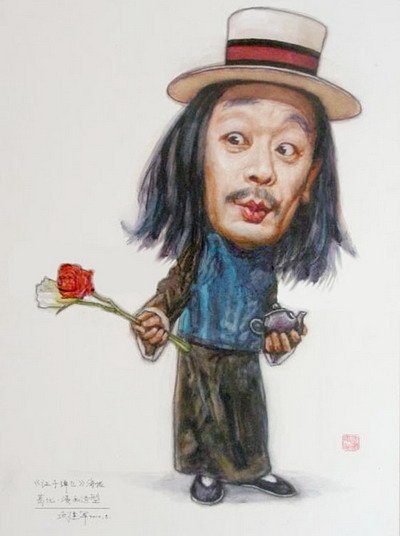
\includegraphics[width=3cm]{ma_bang_de.jpg}
text text

% 图片一般是直接放在一个可以变动的相对位置的环境中,不会像上面那样放在文字之中
\begin{figure}[ht]
    %  figure 环境,就是插图使用的浮动体
    % 环境。figure 环境有可选参数 [ht],表示浮动体可以出现在环境周围的文本所在处
    % (here)和一页的顶部(top)。figure 环境内部相当于普通的段落(默认没有缩进);
    % 第 2 行用声明 \centering 表示后面的内容居中;第 3 行插入图形;第 4 行和第 5 行使
    % 用 \caption 命令给插图加上自动编号和标题;第 6 行的 \label 命令则给图形定义一
    % 个标签,使用这个标签就可以在文章的其他地方引用 \caption 产生的编号(编号引用
    % 我们会在后面讲到)。这段插图的代码非常格式化,在绝大多数情况下,文章中的插图
    % 都是用与这里几乎完全相同的代码插入的。
    \centering
    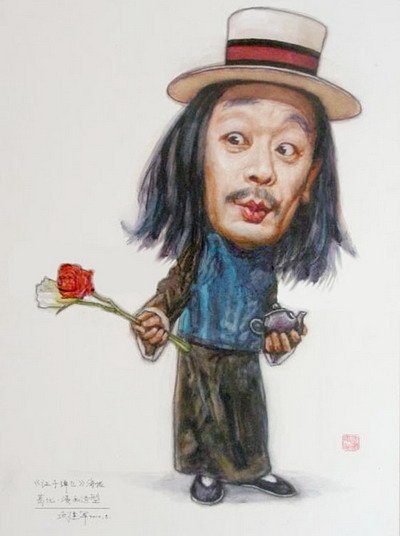
\includegraphics[scale=0.6]{ma_bang_de.jpg}
    \caption{宋赵爽在《周髀算经》注中作的弦图(仿制),该图给出了勾股定理的一个极具对称美的证明。}
    \label{fig:ma_bang_de}

\end{figure}

% 表格
\begin{tabular}{|rrr|}
    % |rrr|表示表格有三列,都是右对齐,在第一列前面和第三列后面各有一条垂直的表格线。在
    % tabular 环境内部,行与行之间用命令 \\ 隔开,每行内部的表项则用符号 & 隔开。表
    % 格中的横线则是用命令 \hline 产生的。
    \hline
    直角边 $a$ & 直角边 $b$ & 斜边 $c$ \\
    \hline
    3       & 4       & 5      \\
    5       & 12      & 13     \\
    8       & 15      & 17     \\
    \hline
\end{tabular}

% 表格和图片的使用方式类似
\begin{table}[H]
    \begin{tabular}{|rrr|}
        \hline
        直角边 $a$ & 直角边 $b$ & 斜边 $c$ \\
        \hline
        3       & 4       & 5      \\
        5       & 12      & 13     \\
        \hline
    \end{tabular}%
    % 命令 \qquad 产生长为 2 em(大约两个“M”的宽度)的空白。
    \qquad
    ($a^2 + b^2 = c^2$)
\end{table}

\section{勾股定理的近代形式}
引用文献 \cite{quanjing}

图 \ref{fig:ma_bang_de} 是我国古代对勾股定理的一种证明 \cite{quanjing}。

\begin{equation}\label{eq:gougu}
    AB^2 = BC^2 + AC^2.
\end{equation}

% 导言区使用 \usepackage{amsmath}
满足式 \eqref{eq:gougu} 的整数称为\emph{勾股数o}。

\nocite{Shiye}
% 的 \bibliographystyle{math} 则是提示 TEX 从文献数据库 math 中获取文献信息,打印参考文献列表
\bibliography{math}



\end{document}


